\section{Reducing Energy Usage Through a New Policy Framework}
\label{sec-reduce}

Redesigning the hardware-software interface will allow next generation
smartphones to effectively allocate energy between components and across time
to meet application needs. Improving performance, however, also requires
prioritizing energy usage to ensure that important applications receive the
resources they need to operate effectively, while recognizing that users use
their phones and applications different and will require different policies.
A user that only charges their phone at night, for example, requires
different energy management strategies than one that charges their phone
regularly at their desk or in the car.

Two major challenges stand in the way of an effective energy management
framework for smartphones. First, while measuring application energy usage
has received a great deal of attention, putting usage into context has not.
Measurement alone may provide helpful feedback to users, but is not
sufficient to enable effective policies, since the behavior and efficiency of
different applications varies, as does their importance to each user. It is
no surprise, for example, that an application like Skype consumes more energy
than a simple messaging client. And this information is not useful on its
own, since Skype's high energy usage might be acceptable if it is often used
and valued and unacceptable if it is not. These uncertainties make energy
usage alone usable for human interpretation---since users can use their own
experience to put the numbers in context---but \textit{unusable} for
automated response or application energy prioritization.

The second challenge is the fact that tuning energy consumption currently
requires deep integration with the specifics of each particular hardware
component, making writing cross-device policies difficult or impossible. A
policy that relies on a certain feature of a Wifi chipset available on a
particular device will fail on a second device if its Wifi driver fails to
support the feature. Without a narrow waste enabling cross-device policies,
energy management improvements will be limited to similar devices and quickly
become obsolete given the rapid improvements in smartphone technologies.

We propose to address both of these challenges through an cross-device energy
management policy framework called \textit{Jouler}. Jouler's policy engine
takes per-application energy measurement and utility determinations and uses
them to select application-specific inefficiency targets. The tuning
component then adjusts component-specific settings to meet the selected
inefficiency target, utilizing the interface improvements achieved by the
redesign objective previously described. To allow policies to be easily moved
between devices, policies do not operate on specific hardware components
directly. Instead, the operate on what we refer to as \textit{idealized
components}, which provide smooth tradeoffs between energy and one of several
performance metrics such as throughput, latency, or fidelity. To be
integrated into Jouler, specific components must translate operations on
these idealized components to adjustments appropriate for their particular
hardware device. Below we describe the two novel contributions of the Jouler
framework---determining application utility and utilizing idealized
components---before describing several possible Jouler policies.

\begin{figure}
  
  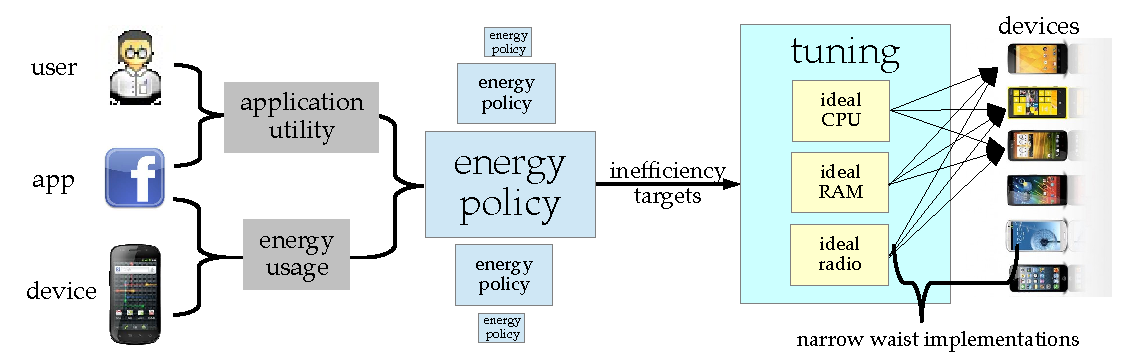
\includegraphics[width=\textwidth]{./figures/jouler.pdf}

  \caption{\textbf{The Jouler energy management policy framework.} Jouler
  addresses two key weaknesses of current smartphone energy management: lack
  of context for application energy usage and inability to write effective
  cross-device policies.}
  
  \vspace*{0.1in}
  \hrule
  \vspace*{-0.1in}
  \label{figure-jouler}

\end{figure}


\subsection{Determining Application Utility}

Smartphone energy modeling provides today's users with easy access to
information about the energy used by the apps running on their device, a
feature incorporated into all major smartphone platforms. However,
prioritizing energy usage between applications requires more information than
just usage statistics. How efficient is the application? How important is it
to the user? What is the relationship between the amount of time it is
actively used and its energy consumption? How sensitive is it to
energy-driven performance degradation? None of these questions can be
answered by only measuring the amount of energy consumed. Usage must be put
into context.

Doing so requires collecting information at the platform level and so will
necessitate changes to the Android sources themselves. Fortunately, our
\PhoneLab{} testbed provides the ability to experiment with platform changes
at scale, which is not currently possible in any other way. (Application
marketplaces do not distribute platform modifications for obvious security
reasons.) We propose to investigate what kinds of information help put energy
usage in context. At a high level, our initial approach is to measure the
amount of information delivered by each application and look at how much
energy is required to do so. Examples of information delivery include
fetching a new email and presenting it to the user, as Gmail would do;
rendering the environment for a game and redrawing the screen, as Angry Birds
would do; or downloading, decoding and rendering a video, as the YouTube
application would do.

Measuring information delivery requires monitoring the interfaces that
smartphones use to deliver content, primarily the display and audio output.
We will then attempt to determine the information content of the stream,
potentially by looking at how compressible it is or using a standard
information theory metric. We may also measure the amount of interaction the
user has with the application, but it is not clear at present if this is
necessary. Simultaneously, we will be measuring the amount of energy the
application is using and provide both as inputs to the Jouler policy
framework. 

\textbf{Our overall goal is to provide a single ratio of energy to
information delivery that measures the efficiency of a broad class of
applications.} Ideally we could use this as direct input into the energy
prioritization process, rewarding applications that deliver a large amount of
content-per-byte and deprioritizing inefficient applications that consume a
great deal of energy but deliver little information.

\subsection{Idealized Components as Narrow Waste for Cross-Device Policies}

Controlling energy usage requires controlling the hardware components that
consume energy, but this is difficult to impossible when each provides a
different interface and to different features. For example, Wifi chipsets on
smartphones provide a variety of potentially-useful energy-performance knobs,
allowing the sleep interval to be altered, power levels adjusted, and
encodings to be changed. Unfortunately, however, not all chipsets support all
of these features, and it is also difficult to reason about how they combine
to affect meaningful performance characteristics such as latency or
throughput.

To address this challenge, Jouler incorporate a novel narrow waste for
implementing energy management utilizing idealized devices. An idealized
device simply trades off energy for some declared performance characteristic
in a smooth, though not necessarily linear, way. When actual components
register with Jouler, they indicate which energy-performance tradeoffs they
can perform. A DVFS memory chip, for example, would declare that it could
trade off throughput for energy usage. Policies in Jouler are then
implemented on top of these idealized components.

Translation between the idealized component and the actual component is done
by a component-specific piece of code that can be implemented by the driver
maintainer or anyone with specific knowledge about that piece of hardware.
\textbf{Thus, Jouler allows energy management policies to be written without
of hardware-specific details and transferred easily between devices.}

\subsection{Policy Framework}

Jouler policies take energy usage and information delivery into account while
operating over the set of idealized components available on a specific
device. We expect that this cross-device energy management framework will
enable many new policies to be developed and shared between users. Users may
experiment with different policies to determine what works best for their
device, or be guided to an appropriate policy through tracing techniques or
usage characterization tools outside the scope of this proposal.

Energy management policies may prioritize energy usage over time, between
applications, or based on any other exogenous information such as the user's
current activity, location, or direct input. Below we provide examples of
several energy management policies that could be implemented in the Jouler
framework.

\begin{itemize}

\item \textbf{Charging pattern adaptation.} Preliminary results on
\PhoneLab{} show that users display varying charging habits. This policy
determines the users charging behavior and then adapts energy usage to try
and devote as much energy to improving application performance while ensuring
that the smartphone will survive until it is plugged in again. The policy may
also prompt periodic chargers based on their location to help them remember
to recharge when power is available. While smartphones are notorious for
running out of energy too soon, arriving at a plug with energy to spare is
also a problem, as that energy could have been used to improve performance.

\item \textbf{Gameplay optimization.} Smartphone games are a
rapidly-expanding segment of the application market. This policy identifies
gameplay and then optimizes the system by allowing the processor and memory
to consume more energy while slowing background tasks and components not
utilized by the game such as storage or networking.

\item \textbf{Rewarding efficient applications.} Not all applications are
implemented efficiently or utilized efficiently by users. This policy uses
the information delivery to energy usage ratio to shift energy towards
applications that are running efficiently. Note that this definition of
energy is appropriately user specific, as it depends on user interaction. An
application that performs a great deal of background caching may be
identified as efficient for a user that uses it often, where the caching pays
off, but simultaneously as inefficient for a user that uses it rarely where
the caching costs are wasted.

\item \textbf{Lower and lower.} This policy simply attempts to reduce
performance for each application until the user reports difficulty using it.
These settings are then saved and reused each time the application is run.
Alternatively, it could provide a kind of energy ``throttle'' allowing users
to speed up or slow down applications interactively at runtime.

\item \textbf{Maximum battery life.} In certain scenarios such as when users
are traveling the time to the next charging opportunity is unknown. In these
situations, all applications must be run as efficiently as possible, and this
can be enabled via a simple Jouler policy.

\end{itemize}

\textbf{By enabling these policies, Jouler facilitates a degree of control
and personalization of energy management not possible today.} We are excited
to see what new policies will emerge once such a policy framework is in
place, and believe that per-user energy management will help keep smartphones
in primary use for longer periods of time thereby improving smartphone
sustainability.
